% Options for packages loaded elsewhere
\PassOptionsToPackage{unicode}{hyperref}
\PassOptionsToPackage{hyphens}{url}
%
\documentclass[
]{article}
\usepackage{amsmath,amssymb}
\usepackage{lmodern}
\usepackage{iftex}
\ifPDFTeX
  \usepackage[T1]{fontenc}
  \usepackage[utf8]{inputenc}
  \usepackage{textcomp} % provide euro and other symbols
\else % if luatex or xetex
  \usepackage{unicode-math}
  \defaultfontfeatures{Scale=MatchLowercase}
  \defaultfontfeatures[\rmfamily]{Ligatures=TeX,Scale=1}
\fi
% Use upquote if available, for straight quotes in verbatim environments
\IfFileExists{upquote.sty}{\usepackage{upquote}}{}
\IfFileExists{microtype.sty}{% use microtype if available
  \usepackage[]{microtype}
  \UseMicrotypeSet[protrusion]{basicmath} % disable protrusion for tt fonts
}{}
\makeatletter
\@ifundefined{KOMAClassName}{% if non-KOMA class
  \IfFileExists{parskip.sty}{%
    \usepackage{parskip}
  }{% else
    \setlength{\parindent}{0pt}
    \setlength{\parskip}{6pt plus 2pt minus 1pt}}
}{% if KOMA class
  \KOMAoptions{parskip=half}}
\makeatother
\usepackage{xcolor}
\usepackage[margin=1in]{geometry}
\usepackage{color}
\usepackage{fancyvrb}
\newcommand{\VerbBar}{|}
\newcommand{\VERB}{\Verb[commandchars=\\\{\}]}
\DefineVerbatimEnvironment{Highlighting}{Verbatim}{commandchars=\\\{\}}
% Add ',fontsize=\small' for more characters per line
\usepackage{framed}
\definecolor{shadecolor}{RGB}{248,248,248}
\newenvironment{Shaded}{\begin{snugshade}}{\end{snugshade}}
\newcommand{\AlertTok}[1]{\textcolor[rgb]{0.94,0.16,0.16}{#1}}
\newcommand{\AnnotationTok}[1]{\textcolor[rgb]{0.56,0.35,0.01}{\textbf{\textit{#1}}}}
\newcommand{\AttributeTok}[1]{\textcolor[rgb]{0.77,0.63,0.00}{#1}}
\newcommand{\BaseNTok}[1]{\textcolor[rgb]{0.00,0.00,0.81}{#1}}
\newcommand{\BuiltInTok}[1]{#1}
\newcommand{\CharTok}[1]{\textcolor[rgb]{0.31,0.60,0.02}{#1}}
\newcommand{\CommentTok}[1]{\textcolor[rgb]{0.56,0.35,0.01}{\textit{#1}}}
\newcommand{\CommentVarTok}[1]{\textcolor[rgb]{0.56,0.35,0.01}{\textbf{\textit{#1}}}}
\newcommand{\ConstantTok}[1]{\textcolor[rgb]{0.00,0.00,0.00}{#1}}
\newcommand{\ControlFlowTok}[1]{\textcolor[rgb]{0.13,0.29,0.53}{\textbf{#1}}}
\newcommand{\DataTypeTok}[1]{\textcolor[rgb]{0.13,0.29,0.53}{#1}}
\newcommand{\DecValTok}[1]{\textcolor[rgb]{0.00,0.00,0.81}{#1}}
\newcommand{\DocumentationTok}[1]{\textcolor[rgb]{0.56,0.35,0.01}{\textbf{\textit{#1}}}}
\newcommand{\ErrorTok}[1]{\textcolor[rgb]{0.64,0.00,0.00}{\textbf{#1}}}
\newcommand{\ExtensionTok}[1]{#1}
\newcommand{\FloatTok}[1]{\textcolor[rgb]{0.00,0.00,0.81}{#1}}
\newcommand{\FunctionTok}[1]{\textcolor[rgb]{0.00,0.00,0.00}{#1}}
\newcommand{\ImportTok}[1]{#1}
\newcommand{\InformationTok}[1]{\textcolor[rgb]{0.56,0.35,0.01}{\textbf{\textit{#1}}}}
\newcommand{\KeywordTok}[1]{\textcolor[rgb]{0.13,0.29,0.53}{\textbf{#1}}}
\newcommand{\NormalTok}[1]{#1}
\newcommand{\OperatorTok}[1]{\textcolor[rgb]{0.81,0.36,0.00}{\textbf{#1}}}
\newcommand{\OtherTok}[1]{\textcolor[rgb]{0.56,0.35,0.01}{#1}}
\newcommand{\PreprocessorTok}[1]{\textcolor[rgb]{0.56,0.35,0.01}{\textit{#1}}}
\newcommand{\RegionMarkerTok}[1]{#1}
\newcommand{\SpecialCharTok}[1]{\textcolor[rgb]{0.00,0.00,0.00}{#1}}
\newcommand{\SpecialStringTok}[1]{\textcolor[rgb]{0.31,0.60,0.02}{#1}}
\newcommand{\StringTok}[1]{\textcolor[rgb]{0.31,0.60,0.02}{#1}}
\newcommand{\VariableTok}[1]{\textcolor[rgb]{0.00,0.00,0.00}{#1}}
\newcommand{\VerbatimStringTok}[1]{\textcolor[rgb]{0.31,0.60,0.02}{#1}}
\newcommand{\WarningTok}[1]{\textcolor[rgb]{0.56,0.35,0.01}{\textbf{\textit{#1}}}}
\usepackage{longtable,booktabs,array}
\usepackage{calc} % for calculating minipage widths
% Correct order of tables after \paragraph or \subparagraph
\usepackage{etoolbox}
\makeatletter
\patchcmd\longtable{\par}{\if@noskipsec\mbox{}\fi\par}{}{}
\makeatother
% Allow footnotes in longtable head/foot
\IfFileExists{footnotehyper.sty}{\usepackage{footnotehyper}}{\usepackage{footnote}}
\makesavenoteenv{longtable}
\usepackage{graphicx}
\makeatletter
\def\maxwidth{\ifdim\Gin@nat@width>\linewidth\linewidth\else\Gin@nat@width\fi}
\def\maxheight{\ifdim\Gin@nat@height>\textheight\textheight\else\Gin@nat@height\fi}
\makeatother
% Scale images if necessary, so that they will not overflow the page
% margins by default, and it is still possible to overwrite the defaults
% using explicit options in \includegraphics[width, height, ...]{}
\setkeys{Gin}{width=\maxwidth,height=\maxheight,keepaspectratio}
% Set default figure placement to htbp
\makeatletter
\def\fps@figure{htbp}
\makeatother
\setlength{\emergencystretch}{3em} % prevent overfull lines
\providecommand{\tightlist}{%
  \setlength{\itemsep}{0pt}\setlength{\parskip}{0pt}}
\setcounter{secnumdepth}{-\maxdimen} % remove section numbering
\ifLuaTeX
  \usepackage{selnolig}  % disable illegal ligatures
\fi
\IfFileExists{bookmark.sty}{\usepackage{bookmark}}{\usepackage{hyperref}}
\IfFileExists{xurl.sty}{\usepackage{xurl}}{} % add URL line breaks if available
\urlstyle{same} % disable monospaced font for URLs
\hypersetup{
  pdftitle={Heart diseases features selection and exploratory data analysis},
  pdfauthor={Wangjun Shen},
  hidelinks,
  pdfcreator={LaTeX via pandoc}}

\title{Heart diseases features selection and exploratory data analysis}
\author{Wangjun Shen}
\date{}

\begin{document}
\maketitle

\hypertarget{introduction}{%
\section{Introduction}\label{introduction}}

The objective of this assignment is to prepare a dataset that can be
used to predict heart disease, a common and serious health issue that
affects a significant portion of the population. The dataset we will be
working on is a subset of a larger real-world dataset collected by
multiple healthcare institutions. It contains various attributes related
to patients' health, such as age, gender, blood pressure, and other
clinical measurements. These attributes can be leveraged to predict the
presence of heart disease.

Data mining plays a critical role in addressing challenges related to
predicting disease spread and similar healthcare problems. By analyzing
large and complex datasets, we can identify patterns and relationships
that may not be immediately apparent. This, in turn, allows us to
develop more accurate predictive models. In the context of heart
disease, data mining techniques can help us extract insights and
patterns from patient data. These insights can aid in identifying risk
factors, predicting disease outcomes, and developing effective treatment
strategies.

For example, by using data mining techniques on the given dataset, we
can identify the most important predictors of heart disease. This
knowledge can then be used to develop a classification model that
accurately predicts the presence of the disease in patients. Moreover,
data mining can also help us identify subpopulations that are more
susceptible to the disease. We can then develop tailored prevention and
treatment strategies for these subpopulations.

Overall, this assignment provides an opportunity to apply data mining
techniques to a real-world dataset. It also allows us to gain hands-on
experience with feature engineering, data exploration, and predictive
modeling. The insights gained from this exploration can inform our work
in subsequent assignments. This, in turn, can help us develop more
accurate and effective predictive models for heart disease and other
similar health challenges.

\hypertarget{related-work}{%
\section{Related Work}\label{related-work}}

\hypertarget{data-exploration}{%
\section{Data Exploration}\label{data-exploration}}

\hypertarget{features-selection}{%
\subsection{Features Selection}\label{features-selection}}

The details of the original dataset are as follows.

\begin{longtable}[]{@{}
  >{\raggedright\arraybackslash}p{(\columnwidth - 4\tabcolsep) * \real{0.3333}}
  >{\raggedright\arraybackslash}p{(\columnwidth - 4\tabcolsep) * \real{0.3333}}
  >{\raggedright\arraybackslash}p{(\columnwidth - 4\tabcolsep) * \real{0.3333}}@{}}
\toprule()
\begin{minipage}[b]{\linewidth}\raggedright
Variable
\end{minipage} & \begin{minipage}[b]{\linewidth}\raggedright
Description
\end{minipage} & \begin{minipage}[b]{\linewidth}\raggedright
Type
\end{minipage} \\
\midrule()
\endhead
id & A unique ID that identifies a participant in the study &
Numerical \\
age & Age in years & Numerical \\
sex & Male and Female were recorded & Categorical \\
cp & Chest Pain type: typical angina; atypical angina; non-anginal pain;
and asymptomatic & Categorical \\
trestbps & Resting blood pressure (in mm Hg on admission to the
hospital) & Numerical \\
chol & Serum Cholestoral in mg/dl & Numerical \\
fbs & Fasting blood sugar \textgreater{} 120 mg/dl (True or False) &
Boolean \\
restecg & Resting electrocardiographic results: normal; having ST-T wave
abnormality (T wave inversions and/or ST elevation or depression of
\textgreater{} 0.05 mV) or showing probable or definite left ventricular
hypertrophy by Estes' criteria & Categorical \\
thalach & Maximum heart rate achieved & Numerical \\
exang & Exercise induced angina (True/False) & Boolean \\
oldpeak & ST depression induced by exercise relative to rest &
Numerical \\
slope & The slope of the peak exercise ST segment: upsloping; flat;
downsloping & Categorical \\
major\_vessels & Number of major vessels (0-3) colored by flourosopy &
Numerical \\
restwm & Rest wall motion abnormality: none; mild or moderate; moderate
or severe; akinesis or dyskmem & Categorical \\
target & Heart disease diagnosed (disease/no disease) & Categorical \\
\bottomrule()
\end{longtable}

Import the dataset and view.

\begin{Shaded}
\begin{Highlighting}[]
\CommentTok{\# load dataset first}
\NormalTok{heart.full }\OtherTok{\textless{}{-}} \FunctionTok{read.csv}\NormalTok{(}\StringTok{"heart.csv"}\NormalTok{)}

\CommentTok{\# then check the dataset}
\FunctionTok{str}\NormalTok{(heart.full)}
\end{Highlighting}
\end{Shaded}

\begin{verbatim}
## 'data.frame':    1025 obs. of  15 variables:
##  $ id           : int  1 2 3 4 5 6 7 8 9 10 ...
##  $ age          : int  52 53 70 61 62 58 58 55 46 54 ...
##  $ sex          : chr  "male" "male" "male" "male" ...
##  $ cp           : chr  "typical angina" "typical angina" "typical angina" "typical angina" ...
##  $ trestbps     : int  125 140 145 148 138 100 114 160 120 122 ...
##  $ chol         : int  212 203 174 203 294 248 318 289 249 286 ...
##  $ fbs          : logi  FALSE TRUE FALSE FALSE TRUE FALSE ...
##  $ restecg      : chr  "ST-T wave abnormality" "normal" "ST-T wave abnormality" "ST-T wave abnormality" ...
##  $ thalach      : int  168 155 125 161 106 122 140 145 144 116 ...
##  $ exang        : logi  FALSE TRUE TRUE FALSE FALSE FALSE ...
##  $ oldpeak      : num  1 3.1 2.6 0 1.9 1 4.4 0.8 0.8 3.2 ...
##  $ slope        : chr  "downsloping" "upsloping" "upsloping" "downsloping" ...
##  $ major_vessels: int  2 0 0 1 3 0 3 1 0 2 ...
##  $ restwm       : chr  "akinesis or dyskmem" "akinesis or dyskmem" "akinesis or dyskmem" "akinesis or dyskmem" ...
##  $ target       : chr  "no disease" "no disease" "no disease" "no disease" ...
\end{verbatim}

From the output results, it can be found that the dataset contains 15
variables and 1025 observation. The details of each variable are
consistent with the description.

Then check the distribution of missing values in the dataset.

\begin{Shaded}
\begin{Highlighting}[]
\FunctionTok{sum}\NormalTok{(}\FunctionTok{is.na}\NormalTok{(heart.full))}
\end{Highlighting}
\end{Shaded}

\begin{verbatim}
## [1] 0
\end{verbatim}

There are not missing values in this data.

The dataset is undergoing a transformation from its original data types
to appropriate data types required for analysis. Originally, the
variables age, trestbps, chol, thalach, and oldpeak were imported as
character vectors representing age, resting blood pressure, serum
cholesterol, maximum heart rate achieved, and ST depression induced by
exercise relative to rest, respectively. These variables have been
converted to a numeric data type since they represent numerical
measurements. Similarly, the variables sex, cp, restecg, slope, restwm,
and target were originally imported as character vectors representing
sex, chest pain type, resting electrocardiographic results, slope of the
peak exercise ST segment, presence of a major vessels colored by
fluoroscopy, and heart disease status, respectively. These variables
have been converted to factor data type since they represent categorical
variables. This transformation allows for easier data manipulation and
analysis, especially when exploring relationships between variables.

\begin{Shaded}
\begin{Highlighting}[]
\CommentTok{\# convert age, trestbps, chol, thalach, and oldpeak to numeric}
\NormalTok{heart.full}\SpecialCharTok{$}\NormalTok{age }\OtherTok{\textless{}{-}} \FunctionTok{as.numeric}\NormalTok{(heart.full}\SpecialCharTok{$}\NormalTok{age)}
\NormalTok{heart.full}\SpecialCharTok{$}\NormalTok{trestbps }\OtherTok{\textless{}{-}} \FunctionTok{as.numeric}\NormalTok{(heart.full}\SpecialCharTok{$}\NormalTok{trestbps)}
\NormalTok{heart.full}\SpecialCharTok{$}\NormalTok{chol }\OtherTok{\textless{}{-}} \FunctionTok{as.numeric}\NormalTok{(heart.full}\SpecialCharTok{$}\NormalTok{chol)}
\NormalTok{heart.full}\SpecialCharTok{$}\NormalTok{thalach }\OtherTok{\textless{}{-}} \FunctionTok{as.numeric}\NormalTok{(heart.full}\SpecialCharTok{$}\NormalTok{thalach)}
\NormalTok{heart.full}\SpecialCharTok{$}\NormalTok{oldpeak }\OtherTok{\textless{}{-}} \FunctionTok{as.numeric}\NormalTok{(heart.full}\SpecialCharTok{$}\NormalTok{oldpeak)}


\CommentTok{\# convert sex, cp, restecg, slope, restwm, and target to factor}
\NormalTok{heart.full}\SpecialCharTok{$}\NormalTok{sex }\OtherTok{\textless{}{-}} \FunctionTok{as.factor}\NormalTok{(heart.full}\SpecialCharTok{$}\NormalTok{sex)}
\NormalTok{heart.full}\SpecialCharTok{$}\NormalTok{cp }\OtherTok{\textless{}{-}} \FunctionTok{as.factor}\NormalTok{(heart.full}\SpecialCharTok{$}\NormalTok{cp)}
\NormalTok{heart.full}\SpecialCharTok{$}\NormalTok{restecg }\OtherTok{\textless{}{-}} \FunctionTok{as.factor}\NormalTok{(heart.full}\SpecialCharTok{$}\NormalTok{restecg)}
\NormalTok{heart.full}\SpecialCharTok{$}\NormalTok{slope }\OtherTok{\textless{}{-}} \FunctionTok{as.factor}\NormalTok{(heart.full}\SpecialCharTok{$}\NormalTok{slope)}
\NormalTok{heart.full}\SpecialCharTok{$}\NormalTok{restwm }\OtherTok{\textless{}{-}} \FunctionTok{as.factor}\NormalTok{(heart.full}\SpecialCharTok{$}\NormalTok{restwm)}
\NormalTok{heart.full}\SpecialCharTok{$}\NormalTok{target }\OtherTok{\textless{}{-}} \FunctionTok{as.factor}\NormalTok{(heart.full}\SpecialCharTok{$}\NormalTok{target)}
\end{Highlighting}
\end{Shaded}

Then use random forest to detect the importance of each feature. In
order to understand whether these features differ between genders, the
data will firstly be created based on the sub-dataset.

\begin{Shaded}
\begin{Highlighting}[]
\CommentTok{\# dataset for each gender}
\NormalTok{heart.male }\OtherTok{\textless{}{-}} \FunctionTok{subset}\NormalTok{(heart.full, sex }\SpecialCharTok{==} \StringTok{"male"}\NormalTok{)}
\NormalTok{heart.female }\OtherTok{\textless{}{-}} \FunctionTok{subset}\NormalTok{(heart.full, sex }\SpecialCharTok{==} \StringTok{"female"}\NormalTok{)}
\end{Highlighting}
\end{Shaded}

Then use those two sub datasets to build the random forest.

For male sub-dataset.

\begin{Shaded}
\begin{Highlighting}[]
\CommentTok{\# Random forest for male subset}
\FunctionTok{library}\NormalTok{(randomForest)}
\end{Highlighting}
\end{Shaded}

\begin{verbatim}
## Warning: package 'randomForest' was built under R version 4.2.2
\end{verbatim}

\begin{verbatim}
## randomForest 4.7-1.1
\end{verbatim}

\begin{verbatim}
## Type rfNews() to see new features/changes/bug fixes.
\end{verbatim}

\begin{Shaded}
\begin{Highlighting}[]
\FunctionTok{set.seed}\NormalTok{(}\DecValTok{123}\NormalTok{)}
\NormalTok{rf\_model\_male }\OtherTok{\textless{}{-}} \FunctionTok{randomForest}\NormalTok{(target }\SpecialCharTok{\textasciitilde{}}\NormalTok{ ., }\AttributeTok{data =}\NormalTok{ heart.male, }\AttributeTok{importance =} \ConstantTok{TRUE}\NormalTok{, }\AttributeTok{ntree =} \DecValTok{500}\NormalTok{)}
\FunctionTok{importance}\NormalTok{(rf\_model\_male)}
\end{Highlighting}
\end{Shaded}

\begin{verbatim}
##                 disease no disease MeanDecreaseAccuracy MeanDecreaseGini
## id             1.606825   3.213858             3.376221        11.154653
## age           33.928469  40.857084            42.838250        34.448119
## sex            0.000000   0.000000             0.000000         0.000000
## cp            38.745483  36.059468            41.121602        47.161819
## trestbps      33.903759  37.024285            41.751265        25.962476
## chol          34.122660  35.756098            39.121768        29.972875
## fbs           16.795603  16.203869            19.636756         3.761825
## restecg       19.083360  19.416802            21.509917         5.531215
## thalach       37.581333  37.899592            43.252118        51.572260
## exang         17.532815  19.401905            20.468760        11.933409
## oldpeak       32.589020  38.902000            40.817055        37.108368
## slope         24.318522  24.566740            27.686364        17.111266
## major_vessels 37.680805  40.115231            43.835239        42.184090
## restwm        31.201322  32.398437            34.984151        25.367047
\end{verbatim}

According to the provided correlation matrix, the most important
features for predicting the presence of heart disease are: cp, thalach,
major\_vessels, oldpeak, trestbps, and age. These features have the
highest correlation with the target variable (disease/no disease), as
well as high values for MeanDecreaseAccuracy and MeanDecreaseGini,
indicating that they are crucial predictors for a machine learning
model.

To facilitate observation, data can be visualized.

\begin{Shaded}
\begin{Highlighting}[]
\FunctionTok{varImpPlot}\NormalTok{(rf\_model\_male, }\AttributeTok{col =} \StringTok{"red"}\NormalTok{, }\AttributeTok{pch =} \DecValTok{20}\NormalTok{)}
\end{Highlighting}
\end{Shaded}

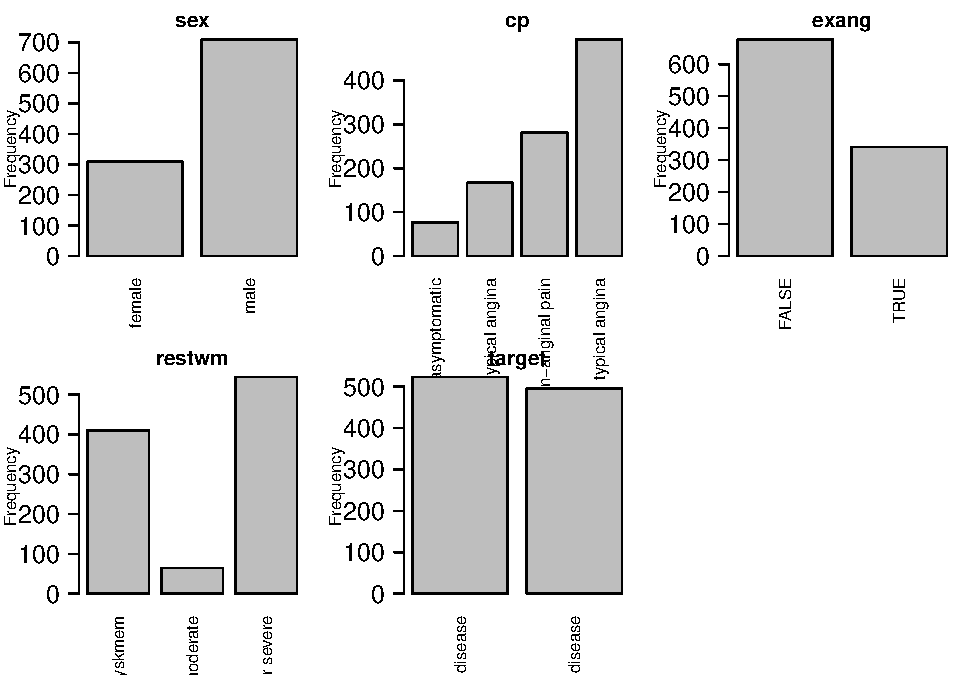
\includegraphics{heart_disease_features_selection_files/figure-latex/unnamed-chunk-6-1.pdf}

The feature chest pain type (cp) has high values for both
MeanDecreaseAccuracy and MeanDecreaseGini, suggesting that it is a
strong predictor for heart disease. Maximum heart rate achieved
(thalach) and the number of major vessels colored by fluoroscopy
(major\_vessels) also have high correlations and values for
MeanDecreaseAccuracy and MeanDecreaseGini, making them strong predictors
as well. Though ST depression induced by exercise relative to rest
(oldpeak) and resting blood pressure (trestbps) have lower correlations,
they still have high values for MeanDecreaseAccuracy and
MeanDecreaseGini, indicating their importance in predicting the presence
of heart disease. Finally, age is also an important feature as it has a
moderate correlation with the target variable and a relatively high
value for MeanDecreaseAccuracy.

In conclusion, these six features can be considered the most important
for predicting the presence of heart disease in males in this dataset.

For female sub-dataset.

\begin{Shaded}
\begin{Highlighting}[]
\CommentTok{\# Random forest for female subset}
\FunctionTok{set.seed}\NormalTok{(}\DecValTok{123}\NormalTok{)}
\NormalTok{rf\_model\_female }\OtherTok{\textless{}{-}} \FunctionTok{randomForest}\NormalTok{(target }\SpecialCharTok{\textasciitilde{}}\NormalTok{ ., }\AttributeTok{data =}\NormalTok{ heart.female, }\AttributeTok{importance =} \ConstantTok{TRUE}\NormalTok{, }\AttributeTok{ntree =} \DecValTok{500}\NormalTok{)}
\FunctionTok{importance}\NormalTok{(rf\_model\_female)}
\end{Highlighting}
\end{Shaded}

\begin{verbatim}
##                 disease no disease MeanDecreaseAccuracy MeanDecreaseGini
## id             1.932703  -3.148355           -0.5202009         2.590325
## age           23.376089  24.724758           28.2364781        12.018921
## sex            0.000000   0.000000            0.0000000         0.000000
## cp            19.702221  20.271296           22.9715941        12.537614
## trestbps      18.409296  18.651176           22.1370717         8.429236
## chol          19.941082  22.898914           25.6314494         8.321454
## fbs            7.611649   9.737944           10.2944996         1.418907
## restecg       14.299858  15.552097           17.3754050         2.982791
## thalach       19.430050  20.969639           24.2566433         8.272732
## exang         18.303884  21.574578           22.6248431         9.167964
## oldpeak       20.677704  21.784792           24.3639560        16.486048
## slope         17.218824  19.973871           21.5111294         8.150365
## major_vessels 19.573486  20.510840           22.7582749        10.407631
## restwm        22.156482  24.907233           26.5256308        22.290165
\end{verbatim}

According to the provided correlation matrix, the following features are
significant in predicting the presence of heart disease in women:

\begin{itemize}
\tightlist
\item
  Age: It exhibits a high correlation with both disease and non-disease
  and has high values for MeanDecreaseAccuracy and MeanDecreaseGini.
\item
  cp (Chest pain type): It exhibits a moderate correlation with disease
  and non-disease, and has high values for MeanDecreaseAccuracy and
  MeanDecreaseGini.
\item
  thalach (Maximum heart rate achieved): It exhibits a moderate
  correlation with disease and non-disease and has high values for
  MeanDecreaseAccuracy and MeanDecreaseGini.
\item
  oldpeak (ST depression induced by exercise relative to rest): It
  exhibits a moderate correlation with disease and non-disease and has a
  high value for MeanDecreaseAccuracy.
\item
  major\_vessels (Number of major vessels (0-3) colored by flourosopy):
  It exhibits a moderate correlation with disease and non-disease and
  has high values for MeanDecreaseAccuracy and MeanDecreaseGini.
\item
  restwm (resting wall motion abnormalities): It exhibits a moderate
  correlation with disease and non-disease and has high values for
  MeanDecreaseAccuracy and MeanDecreaseGini.
\item
  exang (exercise-induced angina): It exhibits a moderate correlation
  with both disease and non-disease and has a high value for
  MeanDecreaseGini.
\end{itemize}

On the other hand, ``trestbps'', ``chol'', ``fbs'', and ``restecg''
display moderate correlations with disease and non-disease but have
relatively lower values for MeanDecreaseAccuracy and MeanDecreaseGini.
As a result, they are not included in the list of important features.

Overall, these seven features are the most significant in predicting the
presence of heart disease in women using this dataset.

To facilitate observation, this is a visualization of the results.

\begin{Shaded}
\begin{Highlighting}[]
\FunctionTok{varImpPlot}\NormalTok{(rf\_model\_female, }\AttributeTok{col =} \StringTok{"red"}\NormalTok{, }\AttributeTok{pch =} \DecValTok{20}\NormalTok{)}
\end{Highlighting}
\end{Shaded}

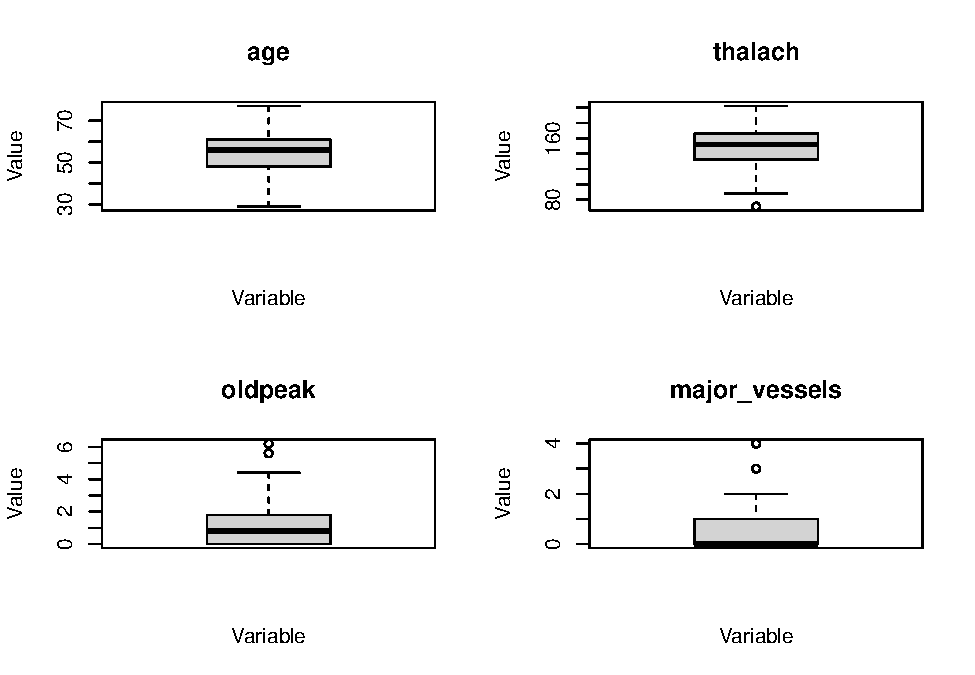
\includegraphics{heart_disease_features_selection_files/figure-latex/unnamed-chunk-8-1.pdf}

Therefore, after comprehensive consideration, we have decided to retain
the following features: age, cp, thalach, oldpeak, major\_vessels,
restwm, exang, and sex.

Now create a new data set with those selected features.

\begin{Shaded}
\begin{Highlighting}[]
\CommentTok{\# Create new dataset with selected features and target variable}
\NormalTok{heart\_features\_selected }\OtherTok{\textless{}{-}}\NormalTok{ heart.full[, }\FunctionTok{c}\NormalTok{(}\StringTok{"id"}\NormalTok{, }\StringTok{"age"}\NormalTok{, }\StringTok{"sex"}\NormalTok{, }\StringTok{"cp"}\NormalTok{, }\StringTok{"thalach"}\NormalTok{, }\StringTok{"exang"}\NormalTok{, }\StringTok{"oldpeak"}\NormalTok{, }\StringTok{"major\_vessels"}\NormalTok{, }\StringTok{"restwm"}\NormalTok{, }\StringTok{"target"}\NormalTok{)]}

\CommentTok{\# Save new dataset as CSV file}
\FunctionTok{write.csv}\NormalTok{(heart\_features\_selected, }\StringTok{"heart\_features\_selected.csv"}\NormalTok{, }\AttributeTok{row.names =} \ConstantTok{FALSE}\NormalTok{)}
\end{Highlighting}
\end{Shaded}

\hypertarget{descriptive-statistics}{%
\subsection{Descriptive Statistics}\label{descriptive-statistics}}

Import the new data set and check the details of that new data set:

\begin{Shaded}
\begin{Highlighting}[]
\NormalTok{heart.selected }\OtherTok{\textless{}{-}} \FunctionTok{read.csv}\NormalTok{(}\StringTok{"heart\_features\_selected.csv"}\NormalTok{)}

\FunctionTok{str}\NormalTok{(heart.selected)}
\end{Highlighting}
\end{Shaded}

\begin{verbatim}
## 'data.frame':    1025 obs. of  10 variables:
##  $ id           : int  1 2 3 4 5 6 7 8 9 10 ...
##  $ age          : int  52 53 70 61 62 58 58 55 46 54 ...
##  $ sex          : chr  "male" "male" "male" "male" ...
##  $ cp           : chr  "typical angina" "typical angina" "typical angina" "typical angina" ...
##  $ thalach      : int  168 155 125 161 106 122 140 145 144 116 ...
##  $ exang        : logi  FALSE TRUE TRUE FALSE FALSE FALSE ...
##  $ oldpeak      : num  1 3.1 2.6 0 1.9 1 4.4 0.8 0.8 3.2 ...
##  $ major_vessels: int  2 0 0 1 3 0 3 1 0 2 ...
##  $ restwm       : chr  "akinesis or dyskmem" "akinesis or dyskmem" "akinesis or dyskmem" "akinesis or dyskmem" ...
##  $ target       : chr  "no disease" "no disease" "no disease" "no disease" ...
\end{verbatim}

Summarize the selected data set.

\begin{Shaded}
\begin{Highlighting}[]
\FunctionTok{library}\NormalTok{(tidyverse)}
\end{Highlighting}
\end{Shaded}

\begin{verbatim}
## Warning: package 'tidyverse' was built under R version 4.2.3
\end{verbatim}

\begin{verbatim}
## Warning: package 'ggplot2' was built under R version 4.2.3
\end{verbatim}

\begin{verbatim}
## Warning: package 'tibble' was built under R version 4.2.3
\end{verbatim}

\begin{verbatim}
## Warning: package 'tidyr' was built under R version 4.2.2
\end{verbatim}

\begin{verbatim}
## Warning: package 'readr' was built under R version 4.2.2
\end{verbatim}

\begin{verbatim}
## Warning: package 'purrr' was built under R version 4.2.2
\end{verbatim}

\begin{verbatim}
## Warning: package 'dplyr' was built under R version 4.2.3
\end{verbatim}

\begin{verbatim}
## Warning: package 'stringr' was built under R version 4.2.2
\end{verbatim}

\begin{verbatim}
## Warning: package 'forcats' was built under R version 4.2.3
\end{verbatim}

\begin{verbatim}
## Warning: package 'lubridate' was built under R version 4.2.3
\end{verbatim}

\begin{verbatim}
## -- Attaching core tidyverse packages ------------------------ tidyverse 2.0.0 --
## v dplyr     1.1.1     v readr     2.1.4
## v forcats   1.0.0     v stringr   1.5.0
## v ggplot2   3.4.2     v tibble    3.2.1
## v lubridate 1.9.2     v tidyr     1.3.0
## v purrr     1.0.1     
## -- Conflicts ------------------------------------------ tidyverse_conflicts() --
## x dplyr::combine()  masks randomForest::combine()
## x dplyr::filter()   masks stats::filter()
## x dplyr::lag()      masks stats::lag()
## x ggplot2::margin() masks randomForest::margin()
## i Use the ]8;;http://conflicted.r-lib.org/conflicted package]8;; to force all conflicts to become errors
\end{verbatim}

\begin{Shaded}
\begin{Highlighting}[]
\NormalTok{heart.selected}\SpecialCharTok{$}\NormalTok{id }\OtherTok{\textless{}{-}} \FunctionTok{as.numeric}\NormalTok{(heart.selected}\SpecialCharTok{$}\NormalTok{id)}
\NormalTok{heart.selected}\SpecialCharTok{$}\NormalTok{age }\OtherTok{\textless{}{-}} \FunctionTok{as.numeric}\NormalTok{(heart.selected}\SpecialCharTok{$}\NormalTok{age)}
\NormalTok{heart.selected}\SpecialCharTok{$}\NormalTok{sex }\OtherTok{\textless{}{-}} \FunctionTok{as.factor}\NormalTok{(heart.selected}\SpecialCharTok{$}\NormalTok{sex)}
\NormalTok{heart.selected}\SpecialCharTok{$}\NormalTok{cp }\OtherTok{\textless{}{-}} \FunctionTok{as.factor}\NormalTok{(heart.selected}\SpecialCharTok{$}\NormalTok{cp)}
\NormalTok{heart.selected}\SpecialCharTok{$}\NormalTok{thalach }\OtherTok{\textless{}{-}} \FunctionTok{as.numeric}\NormalTok{(heart.selected}\SpecialCharTok{$}\NormalTok{thalach)}
\NormalTok{heart.selected}\SpecialCharTok{$}\NormalTok{oldpeak }\OtherTok{\textless{}{-}} \FunctionTok{as.numeric}\NormalTok{(heart.selected}\SpecialCharTok{$}\NormalTok{oldpeak)}
\NormalTok{heart.selected}\SpecialCharTok{$}\NormalTok{major\_vessels }\OtherTok{\textless{}{-}} \FunctionTok{as.numeric}\NormalTok{(heart.selected}\SpecialCharTok{$}\NormalTok{major\_vessels)}
\NormalTok{heart.selected}\SpecialCharTok{$}\NormalTok{target }\OtherTok{\textless{}{-}} \FunctionTok{as.factor}\NormalTok{(heart.selected}\SpecialCharTok{$}\NormalTok{target)}


\FunctionTok{summary}\NormalTok{(heart.selected[, }\SpecialCharTok{{-}}\DecValTok{1}\NormalTok{])}
\end{Highlighting}
\end{Shaded}

\begin{verbatim}
##       age            sex                     cp         thalach     
##  Min.   :29.00   female:312   asymptomatic    : 77   Min.   : 71.0  
##  1st Qu.:48.00   male  :713   atypical angina :167   1st Qu.:132.0  
##  Median :56.00                non-anginal pain:284   Median :152.0  
##  Mean   :54.43                typical angina  :497   Mean   :149.1  
##  3rd Qu.:61.00                                       3rd Qu.:166.0  
##  Max.   :77.00                                       Max.   :202.0  
##    exang            oldpeak      major_vessels       restwm         
##  Mode :logical   Min.   :0.000   Min.   :0.0000   Length:1025       
##  FALSE:680       1st Qu.:0.000   1st Qu.:0.0000   Class :character  
##  TRUE :345       Median :0.800   Median :0.0000   Mode  :character  
##                  Mean   :1.072   Mean   :0.7541                     
##                  3rd Qu.:1.800   3rd Qu.:1.0000                     
##                  Max.   :6.200   Max.   :4.0000                     
##         target   
##  disease   :526  
##  no disease:499  
##                  
##                  
##                  
## 
\end{verbatim}

This result shows the statistical summary of a dataset related to heart
disease. The dataset consists of 1025 observations and several
variables, including age, sex, chest pain type, maximum heart rate,
exercise-induced angina, ST depression induced by exercise relative to
rest, number of major vessels colored by fluoroscopy, and the presence
or absence of heart disease.

The average age of the patients in the dataset is 54.43 years, with a
minimum age of 29 years and a maximum age of 77 years. Out of the 1025
patients, 312 are female and 713 are male. Chest pain type is
categorized into four types, namely asymptomatic, atypical angina,
non-anginal pain, and typical angina. The most frequent type is typical
angina, with 497 occurrences. The maximum heart rate (thalach) ranges
from 71 to 202 beats per minute, with a mean of 149.1 beats per minute.
Exercise-induced angina (exang) is a binary variable, with 345 patients
experiencing it during exercise and 680 patients not experiencing it. ST
depression induced by exercise relative to rest (oldpeak) ranges from 0
to 6.2, with an average value of 1.072. The number of major vessels
colored by fluoroscopy (major\_vessels) ranges from 0 to 4, with a mean
of 0.7541. The dataset is labeled with the presence or absence of heart
disease (target). Out of the 1025 patients, 526 have heart disease and
499 do not have heart disease.

After examining the results, it is clear that there is room for further
analysis. For example, while the report provides some information about
the results, it does not provide a complete picture. In order to gain a
deeper understanding, it would be helpful to explore additional metrics
such as standard deviation, skewness, and kurtosis. This would allow us
to better understand the distribution of the data and identify any
outliers or patterns that may be present. By conducting a more thorough
analysis, we can gain a more comprehensive understanding of the data and
make more informed decisions based on the results.

\begin{Shaded}
\begin{Highlighting}[]
\FunctionTok{library}\NormalTok{(psych)}
\end{Highlighting}
\end{Shaded}

\begin{verbatim}
## Warning: package 'psych' was built under R version 4.2.3
\end{verbatim}

\begin{verbatim}
## 
## Attaching package: 'psych'
\end{verbatim}

\begin{verbatim}
## The following objects are masked from 'package:ggplot2':
## 
##     %+%, alpha
\end{verbatim}

\begin{verbatim}
## The following object is masked from 'package:randomForest':
## 
##     outlier
\end{verbatim}

\begin{Shaded}
\begin{Highlighting}[]
\FunctionTok{describe}\NormalTok{(heart.selected[, }\SpecialCharTok{{-}}\DecValTok{1}\NormalTok{])}
\end{Highlighting}
\end{Shaded}

\begin{verbatim}
## Warning in FUN(newX[, i], ...): no non-missing arguments to min; returning Inf
\end{verbatim}

\begin{verbatim}
## Warning in FUN(newX[, i], ...): no non-missing arguments to max; returning -Inf
\end{verbatim}

\begin{verbatim}
##               vars    n   mean    sd median trimmed   mad min   max range  skew
## age              1 1025  54.43  9.07   56.0   54.66  8.90  29  77.0  48.0 -0.25
## sex*             2 1025   1.70  0.46    2.0    1.74  0.00   1   2.0   1.0 -0.85
## cp*              3 1025   3.17  0.96    3.0    3.31  1.48   1   4.0   3.0 -0.86
## thalach          4 1025 149.11 23.01  152.0  150.40 23.72  71 202.0 131.0 -0.51
## exang            5 1025    NaN    NA     NA     NaN    NA Inf  -Inf  -Inf    NA
## oldpeak          6 1025   1.07  1.18    0.8    0.89  1.19   0   6.2   6.2  1.21
## major_vessels    7 1025   0.75  1.03    0.0    0.57  0.00   0   4.0   4.0  1.26
## restwm*          8 1025   2.14  0.97    3.0    2.17  0.00   1   4.0   3.0 -0.25
## target*          9 1025   1.49  0.50    1.0    1.48  0.00   1   2.0   1.0  0.05
##               kurtosis   se
## age              -0.53 0.28
## sex*             -1.28 0.01
## cp*              -0.39 0.03
## thalach          -0.10 0.72
## exang               NA   NA
## oldpeak           1.29 0.04
## major_vessels     0.68 0.03
## restwm*          -1.81 0.03
## target*          -2.00 0.02
\end{verbatim}

This study provides a summary of the results obtained from a sample of
subjects with different variables related to heart disease. The subjects
had an average age of 54.43 years, with a standard deviation of 9.07.
The majority of subjects were male, with an average value of 1.70 and a
standard deviation of 0.46. The average level of chest pain experienced
by the subjects was 3.17, with a standard deviation of 0.96. The average
maximum heart rate achieved by the subjects was 149.11 bpm, with a
standard deviation of 23.01 bpm. The average ST depression induced by
exercise was 1.07 mm, with a standard deviation of 1.18 mm. The average
number of major vessels colored by fluoroscopy was 0.75, with a standard
deviation of 1.03. The average resting wall motion score index was 2.14,
with a standard deviation of 0.97. The majority of subjects did not have
heart disease, with a mean value of 1.49 and a standard deviation of
0.50. These findings provide important insights into the characteristics
of the sample and may inform future research on heart disease.

\begin{Shaded}
\begin{Highlighting}[]
\FunctionTok{par}\NormalTok{(}\AttributeTok{mfrow=}\FunctionTok{c}\NormalTok{(}\DecValTok{1}\NormalTok{,}\DecValTok{2}\NormalTok{)) }\CommentTok{\# To plot the histograms side by side}
\FunctionTok{hist}\NormalTok{(heart.selected}\SpecialCharTok{$}\NormalTok{age[heart.selected}\SpecialCharTok{$}\NormalTok{sex }\SpecialCharTok{==} \StringTok{"male"}\NormalTok{], }\AttributeTok{main =} \StringTok{"Age Distribution for Males"}\NormalTok{, }\AttributeTok{xlab =} \StringTok{"Age for male"}\NormalTok{)}
\FunctionTok{hist}\NormalTok{(heart.selected}\SpecialCharTok{$}\NormalTok{age[heart.selected}\SpecialCharTok{$}\NormalTok{sex }\SpecialCharTok{==} \StringTok{"female"}\NormalTok{], }\AttributeTok{main =} \StringTok{"Age Distribution for Females"}\NormalTok{, }\AttributeTok{xlab =} \StringTok{"Age for female"}\NormalTok{)}
\end{Highlighting}
\end{Shaded}

\includegraphics{heart_disease_features_selection_files/figure-latex/unnamed-chunk-13-1.pdf}
In terms of male age, the distribution is generally symmetric, or
slightly left-skewed. When compared to the male age distribution, the
female age distribution is more left-skewed. Additionally, it's worth
noting that there are more females over the age of 70 than males.

\begin{Shaded}
\begin{Highlighting}[]
\FunctionTok{boxplot}\NormalTok{(heart.selected}\SpecialCharTok{$}\NormalTok{age }\SpecialCharTok{\textasciitilde{}}\NormalTok{ heart.selected}\SpecialCharTok{$}\NormalTok{target,}
        \AttributeTok{main=}\StringTok{"Heart disease diagnosis distribution by Age"}\NormalTok{,}
         \AttributeTok{ylab=}\StringTok{"Age"}\NormalTok{,}\AttributeTok{xlab=}\StringTok{"Heart disease diagnosed"}\NormalTok{)}
\end{Highlighting}
\end{Shaded}

\includegraphics{heart_disease_features_selection_files/figure-latex/unnamed-chunk-14-1.pdf}

According to our findings, the median age of individuals without disease
is higher than that of those with disease. Moreover, the range in age is
relatively smaller for those without disease. Though there is an outlier
among the no disease group, it is not considered an extreme outlier and
therefore can be retained rather than removed.

\begin{Shaded}
\begin{Highlighting}[]
\FunctionTok{ggplot}\NormalTok{(heart.selected, }\FunctionTok{aes}\NormalTok{(}\AttributeTok{x =}\NormalTok{ target, }\AttributeTok{y =}\NormalTok{ age, }\AttributeTok{fill =}\NormalTok{ sex)) }\SpecialCharTok{+}
  \FunctionTok{geom\_boxplot}\NormalTok{() }\SpecialCharTok{+}
  \FunctionTok{labs}\NormalTok{(}\AttributeTok{title =} \StringTok{"Heart disease diagnosis distribution by Age and Gender"}\NormalTok{,}
       \AttributeTok{x =} \StringTok{"Heart disease diagnosed"}\NormalTok{,}
       \AttributeTok{y =} \StringTok{"Age"}\NormalTok{) }\SpecialCharTok{+}
  \FunctionTok{scale\_fill\_discrete}\NormalTok{(}\AttributeTok{name =} \StringTok{"Sex"}\NormalTok{,}
                      \AttributeTok{labels =} \FunctionTok{c}\NormalTok{(}\StringTok{"Female"}\NormalTok{, }\StringTok{"Male"}\NormalTok{)) }\SpecialCharTok{+}
  \FunctionTok{theme\_minimal}\NormalTok{()}
\end{Highlighting}
\end{Shaded}

\includegraphics{heart_disease_features_selection_files/figure-latex/unnamed-chunk-15-1.pdf}

Females have higher median ages than males, regardless of disease
status. Additionally, it's worth noting that individuals without disease
have a higher average age than those with disease. This may be due to
the fact that individuals with heart disease tend to have shorter
lifespans.

\begin{Shaded}
\begin{Highlighting}[]
\FunctionTok{ggplot}\NormalTok{(}\AttributeTok{data =}\NormalTok{ heart.selected, }\FunctionTok{aes}\NormalTok{(}\AttributeTok{x =}\NormalTok{ target, }\AttributeTok{fill =}\NormalTok{ cp)) }\SpecialCharTok{+} 
  \FunctionTok{geom\_bar}\NormalTok{(}\AttributeTok{position =} \StringTok{"fill"}\NormalTok{) }\SpecialCharTok{+}
  \FunctionTok{labs}\NormalTok{(}\AttributeTok{title =} \StringTok{"Heart disease diagnosis Distributions by Chest pain"}\NormalTok{,}
       \AttributeTok{x =} \StringTok{"Heart disease diagnosis"}\NormalTok{,}
       \AttributeTok{y =} \StringTok{"chest pain"}\NormalTok{) }\SpecialCharTok{+}
  \FunctionTok{theme\_test}\NormalTok{()}
\end{Highlighting}
\end{Shaded}

\includegraphics{heart_disease_features_selection_files/figure-latex/unnamed-chunk-16-1.pdf}

There are four possible outcomes for chest pain (CP), with varying
proportions between individuals with and without the disease. For
individuals with the disease, non-anginal pain has the highest
proportion, followed by atypical angina, while asymptomatic has the
lowest proportion. Conversely, for individuals without the disease,
typical angina has the highest proportion, which is significantly higher
than the proportion in those with the disease, while the other three
types have smaller proportions.

This finding is intriguing because individuals with typical angina
should logically have a higher likelihood of having the disease.
Therefore, further exploration is necessary in subsequent research to
fully understand this relationship.

\begin{Shaded}
\begin{Highlighting}[]
\FunctionTok{mosaicplot}\NormalTok{(heart.selected}\SpecialCharTok{$}\NormalTok{sex }\SpecialCharTok{\textasciitilde{}}\NormalTok{ heart.selected}\SpecialCharTok{$}\NormalTok{target,}
           \AttributeTok{main=}\StringTok{"Heart disease outcome by Gender"}\NormalTok{, }\AttributeTok{shade=}\ConstantTok{FALSE}\NormalTok{,}\AttributeTok{color=}\ConstantTok{TRUE}\NormalTok{,}
           \AttributeTok{xlab=}\StringTok{"Gender"}\NormalTok{, }\AttributeTok{ylab=}\StringTok{"Heart disease"}\NormalTok{)}
\end{Highlighting}
\end{Shaded}

\includegraphics{heart_disease_features_selection_files/figure-latex/unnamed-chunk-17-1.pdf}

Based on the figure above, it is evident that the proportion of disease
is higher among females, while it is relatively low among males. Hence,
it can be inferred that the probability of an observed individual being
classified as having the disease is higher if they are female.

The relationship between CP and disease was examined in different
genders.

\begin{Shaded}
\begin{Highlighting}[]
\CommentTok{\# Create barplot by chest pain and gender}
\FunctionTok{ggplot}\NormalTok{(heart.selected, }\FunctionTok{aes}\NormalTok{(}\AttributeTok{x =}\NormalTok{ target, }\AttributeTok{fill =}\NormalTok{ cp)) }\SpecialCharTok{+}
  \FunctionTok{geom\_bar}\NormalTok{(}\AttributeTok{position =} \StringTok{"fill"}\NormalTok{) }\SpecialCharTok{+}
  \FunctionTok{facet\_wrap}\NormalTok{(}\SpecialCharTok{\textasciitilde{}}\NormalTok{sex) }\SpecialCharTok{+}
  \FunctionTok{labs}\NormalTok{(}\AttributeTok{title =} \StringTok{"Heart disease diagnosis Distributions by Chest pain"}\NormalTok{,}
       \AttributeTok{x =} \StringTok{"Heart disease diagnosis"}\NormalTok{,}
       \AttributeTok{y =} \StringTok{"chest pain"}\NormalTok{) }\SpecialCharTok{+}
  \FunctionTok{scale\_fill\_discrete}\NormalTok{(}\AttributeTok{name =} \StringTok{"Chest Pain"}\NormalTok{) }\SpecialCharTok{+}
  \FunctionTok{theme\_test}\NormalTok{()}
\end{Highlighting}
\end{Shaded}

\includegraphics{heart_disease_features_selection_files/figure-latex/unnamed-chunk-18-1.pdf}

The figure above shows the situation of four types of chest pain under
different genders, which is basically consistent with the overall
results. Therefore, we can conclude that during classification,
regardless of gender, if the observed individual has typical angina,
they are more likely to be classified as having no disease.

The next step involves exploring the Thalach variable visually.

\begin{Shaded}
\begin{Highlighting}[]
\CommentTok{\# Exploratory data analysis of thalach}
\FunctionTok{ggplot}\NormalTok{(}\AttributeTok{data =}\NormalTok{ heart.selected, }\FunctionTok{aes}\NormalTok{(}\AttributeTok{x =}\NormalTok{ thalach)) }\SpecialCharTok{+}
  \FunctionTok{geom\_histogram}\NormalTok{(}\AttributeTok{bins =} \DecValTok{30}\NormalTok{, }\AttributeTok{fill =} \StringTok{"purple"}\NormalTok{, }\AttributeTok{color =} \StringTok{"black"}\NormalTok{) }\SpecialCharTok{+}
  \FunctionTok{labs}\NormalTok{(}\AttributeTok{title =} \StringTok{"Distribution of Maximum Heart Rate Achieved"}\NormalTok{,}
       \AttributeTok{x =} \StringTok{"Maximum Heart Rate Achieved"}\NormalTok{, }\AttributeTok{y =} \StringTok{"Frequency"}\NormalTok{)}
\end{Highlighting}
\end{Shaded}

\includegraphics{heart_disease_features_selection_files/figure-latex/unnamed-chunk-19-1.pdf}
According to the results, the distribution of Thalach exhibits a
slightly skewed left distribution, indicating the possible presence of
an outlier on the left side. However, further analysis is required to
confirm this observation.

\begin{Shaded}
\begin{Highlighting}[]
\FunctionTok{boxplot}\NormalTok{(heart.selected}\SpecialCharTok{$}\NormalTok{thalach }\SpecialCharTok{\textasciitilde{}}\NormalTok{ heart.selected}\SpecialCharTok{$}\NormalTok{target,}
        \AttributeTok{main=}\StringTok{"Heart disease diagnosis distribution by Thalach"}\NormalTok{,}
         \AttributeTok{ylab=}\StringTok{"Thalach"}\NormalTok{,}\AttributeTok{xlab=}\StringTok{"Heart disease diagnosed"}\NormalTok{)}
\end{Highlighting}
\end{Shaded}

\includegraphics{heart_disease_features_selection_files/figure-latex/unnamed-chunk-20-1.pdf}

Based on the figure above, it is evident that the proportion of disease
is higher among females, while it is relatively low among males.
Therefore, it can be inferred that the probability of an observed
individual being classified as having the disease is higher if they are
female.

Moreover, the distribution of thalach for disease appears to be higher
overall than that of no disease, which aligns with common knowledge.
Additionally, there are more outliers for thalach in disease. Thus, it
can be assumed that, in the case of an individual having a relatively
high value of thalach, the probability of them having the disease is
higher, making it easier for them to be classified into the disease
category during classification.

The density diagram below illustrates the distribution of maximum heart
rate achieved for individuals with and without heart disease.

\begin{Shaded}
\begin{Highlighting}[]
\CommentTok{\# Relationship between thalach and target}
\FunctionTok{ggplot}\NormalTok{(}\AttributeTok{data =}\NormalTok{ heart.selected, }\FunctionTok{aes}\NormalTok{(}\AttributeTok{x =}\NormalTok{ thalach, }\AttributeTok{fill =}\NormalTok{ target)) }\SpecialCharTok{+}
  \FunctionTok{geom\_density}\NormalTok{(}\AttributeTok{alpha =} \FloatTok{0.5}\NormalTok{) }\SpecialCharTok{+}
  \FunctionTok{labs}\NormalTok{(}\AttributeTok{title =} \StringTok{"Relationship between Maximum Heart Rate Achieved and Heart Disease Diagnosis"}\NormalTok{,}
       \AttributeTok{x =} \StringTok{"Maximum Heart Rate Achieved"}\NormalTok{, }\AttributeTok{y =} \StringTok{"Density"}\NormalTok{, }\AttributeTok{fill =} \StringTok{"Diagnosis"}\NormalTok{) }\SpecialCharTok{+}
  \FunctionTok{scale\_fill\_manual}\NormalTok{(}\AttributeTok{values =} \FunctionTok{c}\NormalTok{(}\StringTok{"red"}\NormalTok{, }\StringTok{"green"}\NormalTok{))}
\end{Highlighting}
\end{Shaded}

\includegraphics{heart_disease_features_selection_files/figure-latex/unnamed-chunk-21-1.pdf}

The density diagram reveals that, under the condition of having the
disease, the maximum heart rate achieved has higher values and
proportion, which is significantly higher than that of the condition of
no disease. It is suggested that individuals with a higher maximum heart
rate achieved value are more likely to be classified as having the
disease during classification.

\begin{Shaded}
\begin{Highlighting}[]
\CommentTok{\# Relationship between thalach and target divided into gender}
\FunctionTok{ggplot}\NormalTok{(}\AttributeTok{data =}\NormalTok{ heart.selected, }\FunctionTok{aes}\NormalTok{(}\AttributeTok{x =}\NormalTok{ thalach, }\AttributeTok{fill =}\NormalTok{ target)) }\SpecialCharTok{+}
  \FunctionTok{geom\_density}\NormalTok{(}\AttributeTok{alpha =} \FloatTok{0.5}\NormalTok{) }\SpecialCharTok{+}
  \FunctionTok{labs}\NormalTok{(}\AttributeTok{title =} \StringTok{"Relationship between Maximum Heart Rate Achieved and Heart Disease Diagnosis by Gender"}\NormalTok{,}
       \AttributeTok{x =} \StringTok{"Maximum Heart Rate Achieved"}\NormalTok{, }\AttributeTok{y =} \StringTok{"Density"}\NormalTok{, }\AttributeTok{fill =} \StringTok{"Diagnosis"}\NormalTok{) }\SpecialCharTok{+}
  \FunctionTok{scale\_fill\_manual}\NormalTok{(}\AttributeTok{values =} \FunctionTok{c}\NormalTok{(}\StringTok{"red"}\NormalTok{, }\StringTok{"green"}\NormalTok{)) }\SpecialCharTok{+}
  \FunctionTok{facet\_wrap}\NormalTok{(}\SpecialCharTok{\textasciitilde{}}\NormalTok{ sex)}
\end{Highlighting}
\end{Shaded}

\includegraphics{heart_disease_features_selection_files/figure-latex/unnamed-chunk-22-1.pdf}

Regardless of gender, the density of maximum heart rate achieved is very
similar to the overall situation. However, among females with disease,
the proportion of higher maximum heart rate achieved values is very
significant.

Overall, no single variable can make highly accurate predictions, so
combining all variables is necessary for classification.

\hypertarget{correlation-between-variables}{%
\subsection{Correlation Between
Variables}\label{correlation-between-variables}}

To examine the relationship between variables, you can use the cor
function to perform calculations and display the results with a corplot.

\begin{Shaded}
\begin{Highlighting}[]
\CommentTok{\# calculate the correlation matrix}
\FunctionTok{library}\NormalTok{(corrplot)}
\end{Highlighting}
\end{Shaded}

\begin{verbatim}
## Warning: package 'corrplot' was built under R version 4.2.3
\end{verbatim}

\begin{verbatim}
## corrplot 0.92 loaded
\end{verbatim}

\begin{Shaded}
\begin{Highlighting}[]
\NormalTok{heart.selected}\SpecialCharTok{$}\NormalTok{age }\OtherTok{\textless{}{-}} \FunctionTok{as.numeric}\NormalTok{(heart.selected}\SpecialCharTok{$}\NormalTok{age)}
\NormalTok{heart.selected}\SpecialCharTok{$}\NormalTok{thalach }\OtherTok{\textless{}{-}} \FunctionTok{as.numeric}\NormalTok{(heart.selected}\SpecialCharTok{$}\NormalTok{thalach)}
\NormalTok{heart.selected}\SpecialCharTok{$}\NormalTok{oldpeak }\OtherTok{\textless{}{-}} \FunctionTok{as.numeric}\NormalTok{(heart.selected}\SpecialCharTok{$}\NormalTok{oldpeak)}
\NormalTok{heart.selected}\SpecialCharTok{$}\NormalTok{major\_vessels }\OtherTok{\textless{}{-}} \FunctionTok{as.numeric}\NormalTok{(heart.selected}\SpecialCharTok{$}\NormalTok{major\_vessels)}


\NormalTok{cor.matrix }\OtherTok{\textless{}{-}} \FunctionTok{cor}\NormalTok{(heart.selected[, }\FunctionTok{c}\NormalTok{(}\StringTok{"age"}\NormalTok{,  }\StringTok{"thalach"}\NormalTok{, }\StringTok{"oldpeak"}\NormalTok{, }\StringTok{"major\_vessels"}\NormalTok{)])}
\NormalTok{cor.matrix}
\end{Highlighting}
\end{Shaded}

\begin{verbatim}
##                      age    thalach    oldpeak major_vessels
## age            1.0000000 -0.3902271  0.2081367     0.2715505
## thalach       -0.3902271  1.0000000 -0.3497962    -0.2078884
## oldpeak        0.2081367 -0.3497962  1.0000000     0.2218160
## major_vessels  0.2715505 -0.2078884  0.2218160     1.0000000
\end{verbatim}

Age has a positive correlation with major\_vessels (0.2715) and a weak
positive correlation with oldpeak (0.2081). Thalach has a negative
correlation with oldpeak (-0.3498). Finally, oldpeak and major\_vessels
have a moderate positive correlation (0.2218).

\begin{Shaded}
\begin{Highlighting}[]
\FunctionTok{corrplot}\NormalTok{(cor.matrix)}
\end{Highlighting}
\end{Shaded}

\includegraphics{heart_disease_features_selection_files/figure-latex/unnamed-chunk-24-1.pdf}

From the figure, it appears that thalach is negatively correlated with
both age and oldpeak. In terms of positive correlation, major\_vessels
and age appear to be positively correlated.

\end{document}
